%%
%% Elsevier manuscript draft for the MSA--OCV--GBC extension of MixerCSeg.
%% Verified values are traceable to the project logs and generated manifests.
%% Checkpoint selection uses validation data; test data are used once afterward.
%%
\documentclass[preprint,12pt]{elsarticle}

\usepackage{amssymb}
\usepackage{amsmath}
\usepackage{booktabs}
\usepackage{graphicx}
\usepackage{array}
\usepackage{multirow}
\usepackage{url}
\usepackage{float}
\usepackage{xcolor}
\usepackage{tikz}
\usetikzlibrary{arrows.meta,positioning,calc}

\journal{Journal information omitted for review}

\newcommand{\method}{MSA--OCV--GBC}
\newcommand{\R}{\mathbb{R}}
\emergencystretch=2em

\begin{document}

\begin{frontmatter}

\title{Geometry-Aware Crack Segmentation via Multi-Scale Axial Conditioning, Orientation--Curvature Voting, and Gap--Boundary Confidence}

\author[inst1]{Author information omitted for review}
\affiliation[inst1]{organization={Institution information omitted for review}}

\begin{abstract}
Crack segmentation requires a model to preserve elongated structures across scale changes, distinguish true crack ridges from textured background, and recover weak gaps without expanding false-positive regions. This paper presents a geometry-aware extension of MixerCSeg that organizes these requirements into a three-stage refinement chain. A Multi-Scale Axial Conditioner (MSA) first aggregates horizontal, vertical, dilated, row-wise, and column-wise context before the original direction-guided convolution. An Orientation--Curvature Voting module (OCV) then combines first- and second-order differential responses with learnable axial filters to emphasize locally coherent ridges. Finally, a Gap--Boundary Confidence module (GBC) estimates where uncertain features should be retained or bridged from local gap, boundary, and entropy cues. The three modules are integrated by feature-dependent residual gates, yielding the stage order MSA, DEGConv, OCV, and GBC without changing the decoder or training objective. Under validation-only checkpoint selection, four paired CrackMap seeds improve fixed-threshold mIoU from $0.7873\pm0.0212$ to $0.8093\pm0.0093$ and F1 from $0.7438\pm0.0325$ to $0.7763\pm0.0130$. ODS-F1 and OIS-F1 increase from 0.7484 and 0.7545 to 0.7907 and 0.7987, respectively, with positive paired changes for all four seeds. A complete single-seed factorial study shows that OCV--GBC obtains the highest fixed-threshold scores, whereas the full chain obtains the highest ODS/OIS, revealing a threshold-calibration trade-off rather than independent gains from every component. Single-seed transfer improves CamCrack789 but is slightly lower on DeepCrack. The model uses 3.059M parameters and 2.397 GFLOPs, while measured latency increases by 4.4\% over the 2.542M-parameter baseline.
\end{abstract}

\begin{highlights}
\item A three-stage geometry-aware refinement chain is introduced for MixerCSeg.
\item MSA combines multi-scale axial convolution with row and column context.
\item OCV couples Sobel and Hessian evidence with learnable orientation voting.
\item GBC performs confidence-guided feature bridging from gap, boundary, and entropy cues.
\item Validation-selected evaluation reports four paired seeds, full factorial ablation, and controlled transfer to two additional datasets.
\end{highlights}

\begin{keyword}
Crack segmentation \sep Geometry-aware representation \sep Multi-scale axial context \sep Hessian features \sep Boundary confidence \sep Vision Mamba
\end{keyword}

\end{frontmatter}

\section{Introduction}
\label{sec:introduction}

Pixel-level crack maps support pavement assessment, structural health monitoring, and inspection planning. Their extraction remains difficult because crack pixels are sparse, their width changes abruptly, and their visual appearance is easily confused with joints, shadows, stains, and aggregate texture. A successful model must therefore solve three related but distinct problems: it must capture long thin structures at several spatial scales, maintain orientation and curvature consistency, and reconnect weak local evidence without turning background texture into cracks.

Convolutional encoder--decoder networks established strong dense-prediction baselines through hierarchical local features and skip connections~\cite{long2015fcn,ronneberger2015unet}. Crack-specific methods subsequently introduced hierarchical features, boundary modeling, and hybrid convolution--Transformer designs~\cite{zou2019deepcrack,guo2021barnet,xiang2023dtrcnet}. More recently, visual state-space models have offered efficient long-range modeling~\cite{gu2024mamba,liu2024vmamba}. SCSegamba exploits structure-aware scanning for crack topology~\cite{liu2025scsegamba}, while MixerCSeg combines convolutional, Transformer-like, and Mamba-inspired paths with Direction-guided Edge Gated Convolution (DEGConv) and multi-level spatial refinement~\cite{zhao2026mixercseg}. These models substantially improve feature encoding, but difficult samples can still contain scale mismatch, curved ridge ambiguity, and fragmented low-confidence responses.

This work starts from the original MixerCSeg implementation and retains its TransMixer encoder, DEGConv operator, Spatial Refinement Multi-Level Fusion (SRF) decoder, loss definition, and data protocol. Rather than adding another global backbone, we decompose crack-specific refinement into three ordered operations. First, Multi-Scale Axial Conditioning (MSA) supplies DEGConv with learnable horizontal and vertical context at regular and dilated scales, together with global row and column summaries. Second, Orientation--Curvature Voting (OCV) processes the direction-enhanced feature using Sobel and Hessian responses. It favors locations where first-order orientation evidence and ridge-like second-order evidence agree while representing curvature explicitly. Third, Gap--Boundary Confidence (GBC) estimates a spatial confidence map from local feature gaps, boundary contrast, and entropy. This map controls a bridge feature intended to recover weak discontinuities without applying the same correction everywhere.

The modules are not combined by direct addition. Each refinement point uses a learnable, feature-dependent residual gate, and a final stage-level gate returns the refined representation to the original TransMixer feature. The resulting order is
\begin{equation}
\text{TransMixer} \rightarrow \text{MSA} \rightarrow \text{DEGConv}
\rightarrow \text{OCV} \rightarrow \text{GBC} \rightarrow \text{SRF}.
\end{equation}
This order assigns a distinct role to each component: scale conditioning precedes direction extraction, differential voting follows it, and confidence calibration operates on the resulting structural evidence.

The main contributions are as follows:
\begin{itemize}
    \item We introduce MSA, a lightweight conditioner that combines learnable axial depthwise convolutions at two effective scales with row-wise, column-wise, and joint axial context.
    \item We propose OCV, which uses fixed Sobel and Hessian operators to construct magnitude, ridge, curvature, and orientation-voting features before learnable fusion.
    \item We design GBC to infer a spatial bridge confidence from gap, boundary, and entropy cues, and integrate all three modules through gated residual refinement.
    \item We provide validation-selected evaluation on four paired CrackMap seeds and controlled single-seed transfer to DeepCrack and CamCrack789. On CrackMap, the proposed method improves mIoU by 2.20 percentage points, F1 by 3.25 points, ODS-F1 by 4.23 points, and OIS-F1 by 4.42 points on average, with positive paired changes for every seed.
\end{itemize}

\section{Related Work}
\label{sec:related_work}

\subsection{Crack Segmentation}

Traditional crack detection used thresholding, morphology, hand-crafted filters, and structured forests~\cite{shi2016crackforest}. DeepCrack demonstrated that hierarchical convolutional features can capture crack evidence at multiple semantic levels~\cite{zou2019deepcrack}. U-Net-style architectures remain common because high-resolution skip features are useful for narrow structures~\cite{ronneberger2015unet}. Boundary-aware refinement and convolution--Transformer hybrids further improve difficult edges and long-range context~\cite{guo2021barnet,xiang2023dtrcnet}. However, feature aggregation alone does not guarantee that elongated crack fragments remain geometrically consistent.

State-space architectures provide a complementary route to long-range modeling. Mamba introduces input-dependent selective state spaces with linear sequence complexity~\cite{gu2024mamba}, and VMamba adapts selective scanning to hierarchical vision representations~\cite{liu2024vmamba}. CrackMamba studies Mamba from an attention perspective for crack features~\cite{he2024crackmamba}. SCSegamba uses structure-aware scanning and a lightweight gated bottleneck to model crack texture and topology~\cite{liu2025scsegamba}. MixerCSeg, used as the baseline in this work, coordinates local, global, and sequential paths through TransMixer and strengthens irregular edges with DEGConv~\cite{zhao2026mixercseg}. Our method is complementary: it retains this backbone and adds explicit scale, curvature, and confidence reasoning around DEGConv.

\subsection{Axial and Anisotropic Context}

Long, narrow receptive fields are well suited to elongated structures. Strip Pooling showed that $1\times N$ and $N\times1$ operators efficiently capture anisotropic long-range context while reducing interference from unrelated regions~\cite{hou2020strip}. Axial factorization similarly replaces large two-dimensional operations with horizontal and vertical processing. Crack morphology motivates the same inductive bias, but a single axial scale can be insufficient when crack widths and continuity lengths vary. MSA therefore combines standard and dilated axial depthwise convolutions and augments them with full-row and full-column summaries.

\subsection{Differential Geometry and Confidence-Guided Refinement}

First-order gradients describe local edge strength, whereas the Hessian describes second-order variation, principal curvature, and ridge-like structure. Hessian eigen-analysis has long been used to enhance elongated vessels across scales~\cite{frangi1998vessel}. Crack features share a thin curvilinear geometry, although their texture and branching patterns differ from vessels. OCV uses this geometric principle inside a learnable feature block: fixed derivatives provide a stable structural basis, while axial filters and pointwise fusion adapt it to the task.

Uncertainty is also important near thin boundaries and weak fragments. A high-entropy response can indicate an ambiguous feature, while local maxima and local mean differences reveal missing peaks and boundary contrast. GBC combines these cues to decide where a bridge-like correction should contribute. Unlike a purely morphological post-processing step, the confidence map and feature fusion are trained jointly with the segmentation network.

\section{Method}
\label{sec:method}

\subsection{Overall Architecture and Gated Refinement}

Let $\mathbf{X}\in\R^{C\times H\times W}$ be the output of a TransMixer block at one encoder stage. In the baseline, DEGConv directly processes $\mathbf{X}$. In the proposed block, MSA is placed before DEGConv, while OCV and GBC are placed after it. The SRF decoder and segmentation head remain unchanged.

Every optional refinement is integrated through the same residual gate. For an input $\mathbf{A}$ and a refinement function $f$, define
\begin{align}
\mathbf{W}_f &= \sigma\!\left(\psi_f([\mathbf{A};f(\mathbf{A})])\right), \\
\mathcal{G}(\mathbf{A},f;\gamma_f) &=
\mathbf{A}+\gamma_f\mathbf{W}_f\odot\left(f(\mathbf{A})-\mathbf{A}\right),
\label{eq:residual_gate}
\end{align}
where $[\cdot;\cdot]$ denotes channel concatenation, $\psi_f$ is a learnable $1\times1$ convolution, $\sigma$ is the sigmoid function, and $\gamma_f$ is a learnable scalar. The three point-wise scalars are initialized to 0.08. This small initial value limits abrupt feature distortion at the beginning of training.

The block is computed as
\begin{align}
\mathbf{X}_{m} &= \mathcal{G}(\mathbf{X},\mathrm{MSA};\gamma_m), \\
\mathbf{X}_{d} &= \mathrm{DEGConv}(\mathbf{X}_{m}), \\
\mathbf{X}_{o} &= \mathcal{G}(\mathbf{X}_{d},\mathrm{OCV};\gamma_o), \\
\mathbf{X}_{g} &= \mathcal{G}(\mathbf{X}_{o},\mathrm{GBC};\gamma_g), \\
\mathbf{Y} &= \mathcal{G}(\mathbf{X},\mathrm{GN}(\mathbf{X}_{g});\gamma_f),
\label{eq:full_block}
\end{align}
where GN denotes group normalization and the final scalar $\gamma_f$ is initialized to 1.0. Equation~\eqref{eq:full_block} also creates a stage-level residual path from the TransMixer output to the complete geometry-aware refinement.

\begin{figure}[H]
\centering
% Full-width architecture overview with two independent routing bands.
\begingroup
\begin{tikzpicture}[
  x=1cm,
  y=1cm,
  font=\sffamily\footnotesize,
  >=Latex,
  flow/.style={->, line width=0.85pt, draw=black!72},
  feature/.style={->, line width=0.9pt, draw=blue!68!black},
  guidance/.style={->, line width=0.9pt, dashed, draw=orange!86!black},
  band/.style={draw=black!18, rounded corners=2pt, fill=black!1},
  stage/.style={draw=blue!62!black, rounded corners=2pt, fill=blue!6,
    minimum width=20mm, minimum height=13mm, align=center, inner sep=1.5pt},
  merge/.style={draw=black!42, rounded corners=1.5pt, fill=black!4,
    minimum width=5.5mm, minimum height=8mm, align=center, inner sep=1pt},
  projection/.style={draw=teal!65!black, rounded corners=1.5pt, fill=teal!6,
    minimum width=16mm, minimum height=9mm, align=center, inner sep=1.5pt},
  decoder/.style={draw=violet!62!black, rounded corners=1.5pt, fill=violet!6,
    minimum height=10mm, align=center, inner sep=2pt},
  head/.style={draw=orange!78!black, rounded corners=1.5pt, fill=orange!9,
    minimum height=10mm, align=center, inner sep=2pt},
  tap/.style={draw=blue!72!black, fill=blue!12, minimum size=2.8mm, inner sep=0pt},
  note/.style={font=\sffamily\footnotesize, text=black!70}
]

% Encoder band.
\node[band, minimum width=102mm, minimum height=25mm, anchor=south west]
  at (1.95,4.75) {};
\node[font=\sffamily\small\bfseries, anchor=west] at (2.15,6.98)
  {Four-stage encoder};

\node[draw=black!45, fill=white, inner sep=1.0pt] (input) at (0.50,5.60)
  {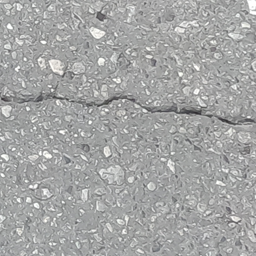
\includegraphics[width=8mm]{../dataset/CrackMap/test_img/GOPR0317 (5).png}};
\node[note, align=center, anchor=north] at ($(input.south)+(0,-0.10)$)
  {Input\\$512^2$};
\node[head, minimum width=9mm] (stem) at (1.55,5.60) {Stem\\$3{\to}16$};

\node[stage] (s1) at (3.05,5.60) {TransMixer\\\textbf{GAB}\\$16,\ 128^2$};
\node[merge] (m1) at (4.40,5.60) {PM\\$\downarrow2$};
\node[stage] (s2) at (5.70,5.60) {TransMixer\\\textbf{GAB}\\$32,\ 64^2$};
\node[merge] (m2) at (7.05,5.60) {PM\\$\downarrow2$};
\node[stage] (s3) at (8.35,5.60) {TransMixer\\\textbf{GAB}\\$64,\ 32^2$};
\node[merge] (m3) at (9.70,5.60) {PM\\$\downarrow2$};
\node[stage] (s4) at (11.00,5.60) {TransMixer\\\textbf{GAB}\\$128,\ 16^2$};

\draw[flow] (input) -- (stem);
\draw[flow] (stem) -- (s1);
\draw[flow] (s1) -- (m1);
\draw[flow] (m1) -- (s2);
\draw[flow] (s2) -- (m2);
\draw[flow] (m2) -- (s3);
\draw[flow] (s3) -- (m3);
\draw[flow] (m3) -- (s4);

% Dedicated vertical ports prevent encoder-to-decoder paths from sharing lines.
\node[tap] (f1) at (3.05,4.42) {};
\node[tap] (f2) at (5.70,4.42) {};
\node[tap] (f3) at (8.35,4.42) {};
\node[tap] (f4) at (11.00,4.42) {};
\node[note, anchor=east] at ($(f1.west)+(-0.05,0)$) {$F_1$};
\node[note, anchor=east] at ($(f2.west)+(-0.05,0)$) {$F_2$};
\node[note, anchor=east] at ($(f3.west)+(-0.05,0)$) {$F_3$};
\node[note, anchor=east] at ($(f4.west)+(-0.05,0)$) {$F_4$};
\draw[feature] (s1.south) -- (f1);
\draw[feature] (s2.south) -- (f2);
\draw[feature] (s3.south) -- (f3);
\draw[feature] (s4.south) -- (f4);

\node[projection] (p1) at (3.05,3.62) {$1{\times}1$ proj.\\$16{\to}8$};
\node[projection] (p2) at (5.70,3.62) {$1{\times}1$ proj.\\$32{\to}8$};
\node[projection] (p3) at (8.35,3.62) {$1{\times}1$ proj.\\$64{\to}8$};
\node[projection] (p4) at (11.00,3.62) {$1{\times}1$ proj.\\$128{\to}8$};
\draw[feature] (f1) -- (p1);
\draw[feature] (f2) -- (p2);
\draw[feature] (f3) -- (p3);
\draw[feature] (f4) -- (p4);

% Decoder band.
\node[band, draw=violet!22, fill=violet!1, minimum width=129mm,
  minimum height=32mm, anchor=south west] at (0.35,-0.25) {};
\node[font=\sffamily\small\bfseries, text=violet!68!black, anchor=east]
  at (13.05,2.70) {SRF decoder};

\node[decoder, minimum width=19mm] (up1) at (1.52,2.02)
  {$F_1$ upsample\\to $512^2$};
\node[decoder, minimum width=21mm] (att) at (3.88,2.02)
  {Spatial attention\\$A=\sigma(\phi(F_1))$};
\node[decoder, minimum width=32mm] (align) at (7.30,2.02)
  {Align $F_{2:4}$ to $128^2$\\calibrate by $A$, then upsample};
\node[decoder, minimum width=14mm] (cat) at (7.30,0.72) {Concat\\$32$ ch};
\node[decoder, minimum width=16mm] (fuse) at (9.15,0.72)
  {Conv + GN\\$32{\to}8$};
\node[head, minimum width=14mm] (pred) at (10.92,0.72)
  {Prediction\\head};
\node[draw=black!45, fill=white, inner sep=1.0pt] (output) at (12.32,0.72)
  {\includegraphics[width=7.5mm]{../results/probability_maps/triple_stack_v4_crackmap/validate_v3_msa_ocv_gbc_seed42/GOPR0317 (5)_pre.png}};
\node[note, align=center, anchor=north] at ($(output.south)+(0,-0.09)$)
  {Probability map};

\draw[feature] (p1.south) -- ++(0,-0.20) -| (up1.north);
\draw[guidance] (p1.south east) -- ++(0,-0.38) -| (att.north);
\draw[feature] (p2.south) -- ++(0,-0.48) -| ([xshift=2mm]align.north west);
\draw[feature] (p3.south) -- ++(0,-0.31) -| (align.north);
\draw[feature] (p4.south) -- ++(0,-0.14) -| ([xshift=-2mm]align.north east);
\draw[guidance] (att.east) -- (align.west);
\draw[feature] (up1.south) -- ++(0,-0.55) -| (cat.west);
\draw[feature] (align.south) -- (cat.north);
\draw[flow] (cat) -- (fuse);
\draw[flow] (fuse) -- (pred);
\draw[flow] (pred) -- (output);

% Legend outside the data paths.
\draw[feature] (0.10,-0.52) -- (0.65,-0.52);
\node[note, anchor=west] at (0.72,-0.52) {feature};
\draw[guidance] (2.05,-0.52) -- (2.60,-0.52);
\node[note, anchor=west] at (2.67,-0.52) {$F_1$ guidance};

\end{tikzpicture}
\endgroup

\caption{Overall architecture of MSA--OCV--GBC MixerCSeg. The four encoder stages retain TransMixer and insert a geometry-aware block (GAB) around the inherited DEGConv path. Multi-level features $F_1$--$F_4$ are projected to eight channels; $F_1$ supplies spatial guidance for calibrating $F_2$--$F_4$ before full-resolution fusion. The input and output are from the same seed-42 CrackMap example.}
\label{fig:architecture}
\end{figure}

Figure~\ref{fig:gab_visual} expands the GAB inserted after every TransMixer. The four encoder stages use channels $[16,32,64,128]$ and resolutions from $128\times128$ to $16\times16$. Each GAB follows the same MSA--DEGConv--OCV--GBC topology but uses stage-specific parameters and channel widths. Feature-dependent residual gates control the three local refinements, while the final gate preserves a stage-level identity route.

\begin{figure}[H]
\centering
% Exact TripleStackV3Block data flow, unfolded into three spacious rows.
\begingroup
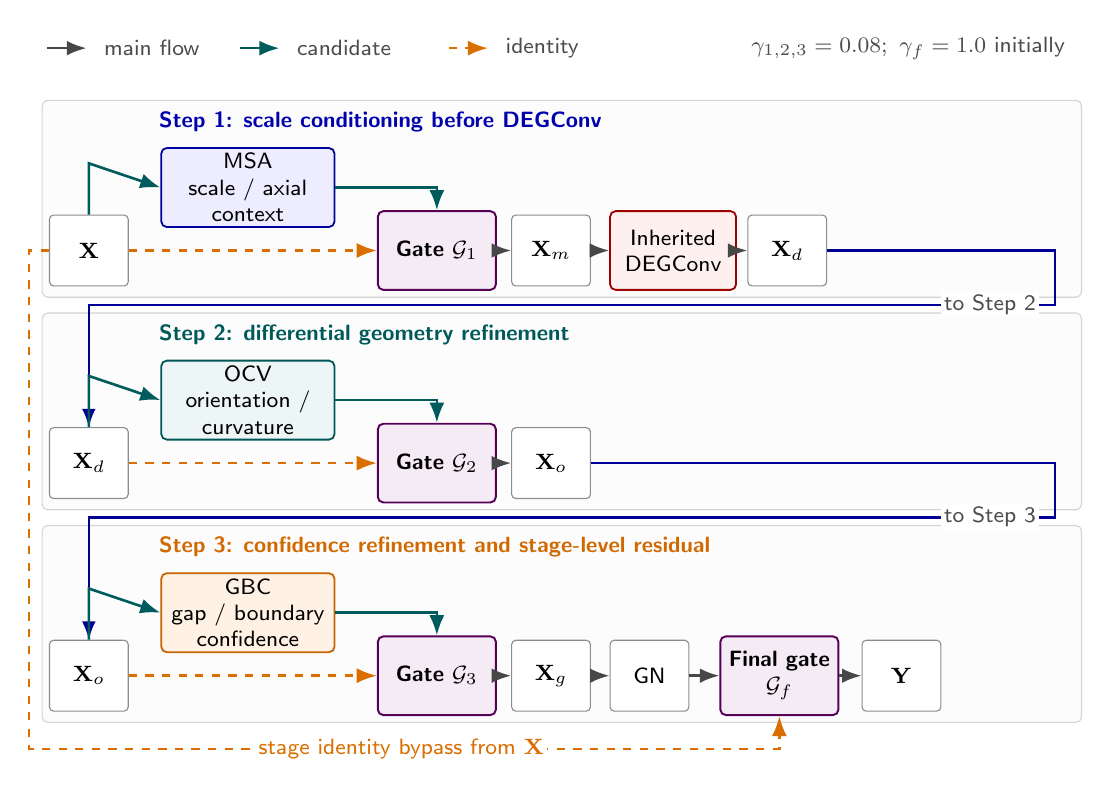
\begin{tikzpicture}[
  x=1cm,
  y=1cm,
  font=\sffamily\footnotesize,
  >=Latex,
  flow/.style={->, line width=0.9pt, draw=black!72},
  candidate/.style={->, line width=0.95pt, draw=teal!72!black},
  identity/.style={->, line width=0.95pt, dashed, draw=orange!86!black},
  transfer/.style={->, line width=0.8pt, draw=blue!58!black},
  band/.style={draw=black!17, rounded corners=2pt, fill=black!1},
  module/.style={rounded corners=2pt, minimum width=22mm, minimum height=10mm,
    align=center, inner sep=2pt, line width=0.65pt},
  msa/.style={module, draw=blue!62!black, fill=blue!7},
  ocv/.style={module, draw=teal!67!black, fill=teal!7},
  gbc/.style={module, draw=orange!78!black, fill=orange!10},
  inherited/.style={module, minimum width=16mm, draw=red!62!black, fill=red!6},
  gate/.style={draw=violet!68!black, fill=violet!8, rounded corners=2pt,
    minimum width=15mm, minimum height=10mm, align=center, inner sep=1.5pt,
    line width=0.7pt, font=\sffamily\footnotesize\bfseries},
  tensor/.style={draw=black!45, fill=white, rounded corners=1.5pt,
    minimum width=10mm, minimum height=9mm, align=center, inner sep=1.5pt},
  note/.style={font=\sffamily\footnotesize, text=black!70},
  rowtitle/.style={font=\sffamily\footnotesize\bfseries, anchor=west}
]

% Legend is isolated above the computational graph.
\draw[flow] (0.25,8.72) -- (0.75,8.72);
\node[note, anchor=west] at (0.85,8.72) {main flow};
\draw[candidate] (2.70,8.72) -- (3.20,8.72);
\node[note, anchor=west] at (3.30,8.72) {candidate};
\draw[identity] (5.35,8.72) -- (5.85,8.72);
\node[note, anchor=west] at (5.95,8.72) {identity};
\node[note, anchor=east] at (13.30,8.72)
  {$\gamma_{1,2,3}=0.08;\ \gamma_f=1.0$ initially};

% Step 1: MSA gate followed by the inherited DEGConv.
\node[band, minimum width=132mm, minimum height=25mm, anchor=south west]
  at (0.18,5.55) {};
\node[rowtitle, text=blue!68!black] at (1.55,7.78)
  {Step 1: scale conditioning before DEGConv};
\node[tensor] (x) at (0.78,6.15) {$\mathbf{X}$};
\node[msa] (msa) at (2.80,6.95) {MSA\\scale / axial\\context};
\node[gate] (g1) at (5.20,6.15) {Gate $\mathcal{G}_1$};
\node[tensor] (xm) at (6.65,6.15) {$\mathbf{X}_m$};
\node[inherited] (deg) at (8.20,6.15) {Inherited\\DEGConv};
\node[tensor] (xd) at (9.65,6.15) {$\mathbf{X}_d$};
\draw[identity] (x.east) -- (g1.west);
\draw[candidate] (x.north) -- ++(0,0.65) -- (msa.west);
\draw[candidate] (msa.east) -- ++(0.45,0) -| (g1.north);
\draw[flow] (g1) -- (xm);
\draw[flow] (xm) -- (deg);
\draw[flow] (deg) -- (xd);

% Step 2: orientation and curvature vote.
\node[band, minimum width=132mm, minimum height=25mm, anchor=south west]
  at (0.18,2.85) {};
\node[rowtitle, text=teal!70!black] at (1.55,5.08)
  {Step 2: differential geometry refinement};
% Draw the receiving node after the band so that the background cannot cover it.
\node[tensor] (xd2) at (0.78,3.45) {$\mathbf{X}_d$};
\draw[transfer] (xd.east) -- (13.05,6.15) -- (13.05,5.46)
  -- (0.78,5.46) -- (xd2.north);
\node[note, anchor=east, fill=white, inner sep=1pt] at (12.85,5.46)
  {to Step 2};
\node[ocv] (ocv) at (2.80,4.25) {OCV\\orientation /\\curvature};
\node[gate] (g2) at (5.20,3.45) {Gate $\mathcal{G}_2$};
\node[tensor] (xo) at (6.65,3.45) {$\mathbf{X}_o$};
\draw[identity] (xd2.east) -- (g2.west);
\draw[candidate] (xd2.north) -- ++(0,0.65) -- (ocv.west);
\draw[candidate] (ocv.east) -- ++(0.45,0) -| (g2.north);
\draw[flow] (g2) -- (xo);

% Step 3: gap confidence, normalization, and the stage-level gate.
\node[band, minimum width=132mm, minimum height=25mm, anchor=south west]
  at (0.18,0.15) {};
\node[rowtitle, text=orange!82!black] at (1.55,2.38)
  {Step 3: confidence refinement and stage-level residual};
% Draw the receiving node after the band so that the background cannot cover it.
\node[tensor] (xo2) at (0.78,0.75) {$\mathbf{X}_o$};
\draw[transfer] (xo.east) -- (13.05,3.45) -- (13.05,2.76)
  -- (0.78,2.76) -- (xo2.north);
\node[note, anchor=east, fill=white, inner sep=1pt] at (12.85,2.76)
  {to Step 3};
\node[gbc] (gbc) at (2.80,1.55) {GBC\\gap / boundary\\confidence};
\node[gate] (g3) at (5.20,0.75) {Gate $\mathcal{G}_3$};
\node[tensor] (xg) at (6.65,0.75) {$\mathbf{X}_g$};
\node[tensor, minimum width=10mm] (gn) at (7.90,0.75) {GN};
\node[gate] (gf) at (9.55,0.75) {Final gate\\$\mathcal{G}_f$};
\node[tensor] (y) at (11.10,0.75) {$\mathbf{Y}$};
\draw[identity] (xo2.east) -- (g3.west);
\draw[candidate] (xo2.north) -- ++(0,0.65) -- (gbc.west);
\draw[candidate] (gbc.east) -- ++(0.45,0) -| (g3.north);
\draw[flow] (g3) -- (xg);
\draw[flow] (xg) -- (gn);
\draw[flow] (gn) -- (gf);
\draw[flow] (gf) -- (y);

% Stage identity remains on its own outer lane.
\draw[identity] (x.west) -- (0.02,6.15) -- (0.02,-0.18)
  -- (9.55,-0.18) -- (gf.south);
\node[note, text=orange!86!black, fill=white, inner sep=1pt]
  at (4.75,-0.18) {stage identity bypass from $\mathbf{X}$};

\end{tikzpicture}
\endgroup

\caption{Exact GAB data flow. Each local gate receives both an identity feature (dashed orange) and a candidate refinement (teal): MSA is gated before the inherited DEGConv, whereas OCV and GBC are gated afterward. Group normalization precedes the final stage-level gate $\mathcal{G}_f$, which also receives the original TransMixer feature. The displayed order and gate initializations match the implementation.}
\label{fig:gab_visual}
\end{figure}

\subsection{Multi-Scale Axial Conditioner}
\label{sec:msa}

MSA addresses the scale and anisotropy of crack structures before direction-guided processing. Four depthwise branches operate on $\mathbf{X}$:
\begin{align}
\mathbf{A}_{h} &= \phi^{dw}_{1\times9}(\mathbf{X}), &
\mathbf{A}_{v} &= \phi^{dw}_{9\times1}(\mathbf{X}), \\
\mathbf{A}_{dh} &= \phi^{dw}_{1\times5,d=2}(\mathbf{X}), &
\mathbf{A}_{dv} &= \phi^{dw}_{5\times1,d=2}(\mathbf{X}),
\end{align}
where each $\phi$ contains depthwise convolution, group normalization, and SiLU activation. The axial response is
\begin{equation}
\mathbf{A}=\mathbf{A}_{h}+\mathbf{A}_{v}+\mathbf{A}_{dh}+\mathbf{A}_{dv}.
\end{equation}
The regular branches capture nearby elongated patterns, while dilation enlarges the effective support without a dense square kernel.

MSA also forms row and column descriptors:
\begin{align}
\mathbf{R}_{c,i,j} &= \frac{1}{W}\sum_{q=1}^{W}\mathbf{X}_{c,i,q}, \\
\mathbf{C}_{c,i,j} &= \frac{1}{H}\sum_{p=1}^{H}\mathbf{X}_{c,p,j},
\end{align}
where the reduced dimension is broadcast back to $H\times W$. Their product $\mathbf{R}\odot\mathbf{C}$ encodes positions jointly supported by horizontal and vertical context. The conditioned feature is
\begin{equation}
\mathrm{MSA}(\mathbf{X})=\phi_{1\times1}
([\mathbf{X};\mathbf{A};\mathbf{R};\mathbf{C};\mathbf{R}\odot\mathbf{C}]).
\label{eq:msa}
\end{equation}

\subsection{Orientation--Curvature Voting}
\label{sec:ocv}

OCV processes $\mathbf{X}_d$ after DEGConv. Fixed Sobel kernels produce horizontal and vertical gradients $\mathbf{g}_x$ and $\mathbf{g}_y$, with magnitude
\begin{equation}
\mathbf{M}=\sqrt{\mathbf{g}_x^2+\mathbf{g}_y^2+\epsilon}.
\end{equation}
Second-order derivative kernels produce $\mathbf{D}_{xx}$, $\mathbf{D}_{yy}$, and $\mathbf{D}_{xy}$. We define a ridge-strength proxy
\begin{equation}
\boldsymbol{\rho}=\sqrt{(\mathbf{D}_{xx}-\mathbf{D}_{yy})^2+4\mathbf{D}_{xy}^{2}+\epsilon},
\label{eq:ridge}
\end{equation}
and a curvature-magnitude proxy
\begin{equation}
\boldsymbol{\kappa}=\sqrt{(\mathbf{D}_{xx}+\mathbf{D}_{yy})^2+\mathbf{D}_{xy}^{2}+\epsilon}.
\label{eq:curvature}
\end{equation}
These expressions are related to the discriminant and trace of the local Hessian and supply complementary evidence about anisotropy and bending.

Learnable $1\times7$ and $7\times1$ depthwise filters provide horizontal and vertical features. Their contributions are selected by gradient orientation:
\begin{align}
\mathbf{H} &= \sigma(|\mathbf{g}_x|-|\mathbf{g}_y|)\odot
\phi^{dw}_{1\times7}(\mathbf{X}_{d}), \\
\mathbf{V} &= \sigma(|\mathbf{g}_y|-|\mathbf{g}_x|)\odot
\phi^{dw}_{7\times1}(\mathbf{X}_{d}).
\end{align}
The geometry vote is
\begin{equation}
\mathbf{Q}=\sigma(\boldsymbol{\rho}-\boldsymbol{\kappa})\odot(\mathbf{H}+\mathbf{V}),
\end{equation}
which emphasizes axial evidence when the ridge response dominates the curvature proxy. Finally,
\begin{equation}
\mathrm{OCV}(\mathbf{X}_{d})=\phi_{1\times1}
([\mathbf{X}_{d};\mathbf{M};\boldsymbol{\rho};\boldsymbol{\kappa};\mathbf{Q}]).
\label{eq:ocv}
\end{equation}

\subsection{Gap--Boundary Confidence}
\label{sec:gbc}

GBC decides where a local bridging response should replace uncertain evidence. Given $\mathbf{X}_o$, the feature probability and binary entropy are
\begin{align}
\mathbf{P} &= \sigma(\mathbf{X}_{o}), \\
\mathbf{E} &= -\mathbf{P}\log(\mathbf{P}+\epsilon)
-(1-\mathbf{P})\log(1-\mathbf{P}+\epsilon).
\end{align}
We compute a $3\times3$ local mean $\bar{\mathbf{X}}_o$, a non-negative local gap response, and boundary contrast:
\begin{align}
\boldsymbol{\Delta} &= \max\!\left(
\mathrm{MaxPool}_{5\times5}(\mathbf{X}_o)-\mathbf{X}_o,0\right), \\
\mathbf{B} &= |\mathbf{X}_o-\bar{\mathbf{X}}_o|.
\end{align}
The spatial confidence map uses channel summaries of the three cues:
\begin{equation}
\mathbf{C}_{g}=\sigma\!\left(
\psi_{5\times5}
([\max_c\boldsymbol{\Delta};\operatorname{mean}_c\mathbf{B};
\operatorname{mean}_c\mathbf{E}])\right).
\label{eq:confidence}
\end{equation}
It controls the bridge feature
\begin{equation}
\mathbf{Z}=\mathbf{X}_o\odot(1-\mathbf{C}_{g})+
\boldsymbol{\Delta}\odot\mathbf{C}_{g}.
\end{equation}
The GBC output is then
\begin{equation}
\mathrm{GBC}(\mathbf{X}_o)=\phi_{1\times1}
([\mathbf{X}_o;\boldsymbol{\Delta};\mathbf{B};\mathbf{E};\mathbf{Z}]).
\label{eq:gbc}
\end{equation}
Thus, bridging is spatially modulated rather than uniformly applied.

Figures~\ref{fig:msa_detail}--\ref{fig:gbc_detail} expand the branch topology of the three proposed modules. The modules are separated into full-width diagrams so that every branch, fusion input, and unchanged identity route remains visible at the final manuscript scale. The shared residual gate and its placement are shown separately in Fig.~\ref{fig:gab_visual}.

\begin{figure}[H]
\centering
% Multi-Scale Axial Conditioner with one route per branch.
\begingroup
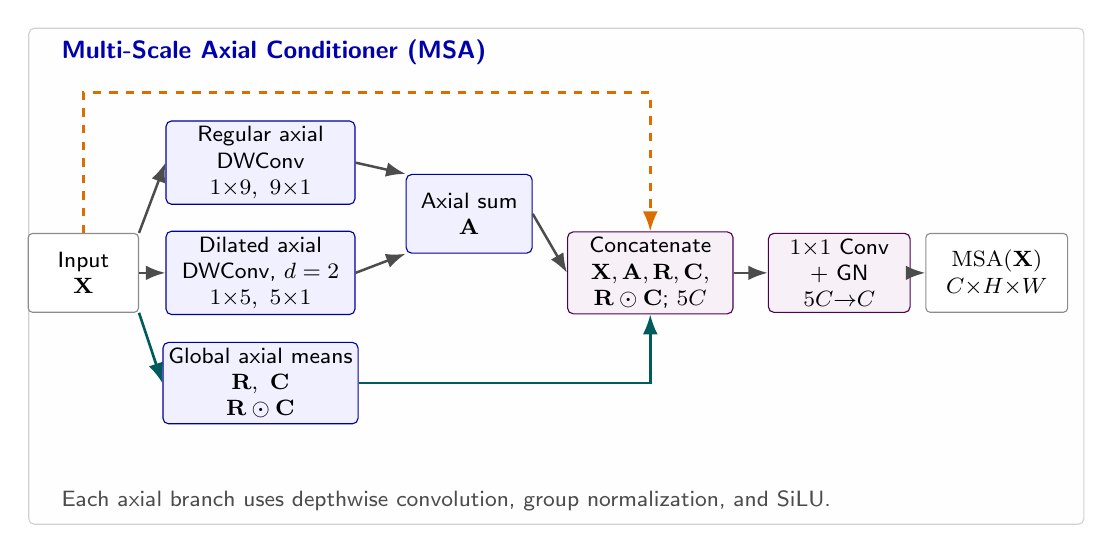
\begin{tikzpicture}[
  x=1cm,
  y=1cm,
  font=\sffamily\footnotesize,
  >=Latex,
  flow/.style={->, line width=0.9pt, draw=black!70},
  cue/.style={->, line width=0.95pt, draw=teal!72!black},
  skip/.style={->, line width=0.95pt, dashed, draw=orange!86!black},
  panel/.style={draw=black!18, rounded corners=2pt, fill=black!0.5},
  io/.style={draw=black!45, fill=white, rounded corners=1.5pt,
    minimum width=14mm, minimum height=10mm, align=center, inner sep=2pt},
  op/.style={draw=blue!62!black, fill=blue!6, rounded corners=2pt,
    minimum height=10mm, align=center, inner sep=2pt},
  fusion/.style={draw=violet!62!black, fill=violet!6, rounded corners=2pt,
    minimum height=10mm, align=center, inner sep=2pt},
  note/.style={font=\sffamily\footnotesize, text=black!70}
]

\node[panel, minimum width=134mm, minimum height=63mm, anchor=south west]
  at (0.05,0.05) {};
\node[font=\sffamily\small\bfseries, text=blue!68!black, anchor=west]
  at (0.35,6.05) {Multi-Scale Axial Conditioner (MSA)};

\node[io] (x) at (0.75,3.25) {Input\\$\mathbf{X}$};
\node[op, minimum width=24mm] (regular) at (3.00,4.65)
  {Regular axial\\DWConv\\$1{\times}9,\ 9{\times}1$};
\node[op, minimum width=24mm] (dilated) at (3.00,3.25)
  {Dilated axial\\DWConv, $d=2$\\$1{\times}5,\ 5{\times}1$};
\node[op, minimum width=24mm] (context) at (3.00,1.85)
  {Global axial means\\$\mathbf{R},\ \mathbf{C}$\\$\mathbf{R}\odot\mathbf{C}$};
\node[op, minimum width=16mm] (sum) at (5.65,4.00)
  {Axial sum\\$\mathbf{A}$};
\node[fusion, minimum width=21mm] (concat) at (7.95,3.25)
  {Concatenate\\$\mathbf{X},\mathbf{A},\mathbf{R},\mathbf{C},$\\$\mathbf{R}\odot\mathbf{C}$; $5C$};
\node[fusion, minimum width=18mm] (fuse) at (10.35,3.25)
  {$1{\times}1$ Conv\\+ GN\\$5C{\to}C$};
\node[io, minimum width=18mm] (out) at (12.35,3.25)
  {$\mathrm{MSA}(\mathbf{X})$\\$C{\times}H{\times}W$};

\draw[flow] (x.north east) -- (regular.west);
\draw[flow] (x.east) -- (dilated.west);
\draw[cue] (x.south east) -- (context.west);
\draw[flow] (regular.east) -- (sum.north west);
\draw[flow] (dilated.east) -- (sum.south west);
\draw[flow] (sum.east) -- (concat.west);
\draw[cue] (context.east) -- ++(0.42,0) -| (concat.south);
\draw[skip] (x.north) -- ++(0,1.78) -| (concat.north);
\draw[flow] (concat) -- (fuse);
\draw[flow] (fuse) -- (out);

\node[note, anchor=west] at (0.35,0.35)
  {Each axial branch uses depthwise convolution, group normalization, and SiLU.};

\end{tikzpicture}
\endgroup

\caption{Implementation-level MSA data flow. Regular and dilated axial depthwise branches form $\mathbf{A}$, while row, column, and joint axial summaries enter the final $5C$-channel fusion through a separate route. The dashed orange path carries the unchanged input.}
\label{fig:msa_detail}
\end{figure}

\begin{figure}[H]
\centering
% Orientation--Curvature Voting with separated derivative and voting lanes.
\begingroup
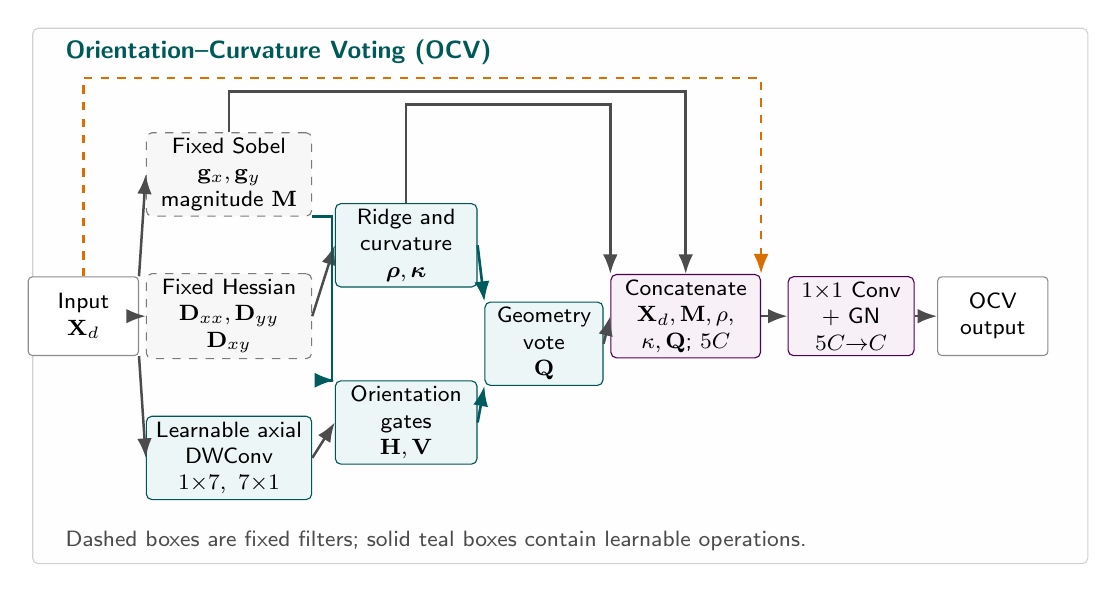
\begin{tikzpicture}[
  x=1cm,
  y=1cm,
  font=\sffamily\footnotesize,
  >=Latex,
  flow/.style={->, line width=0.9pt, draw=black!70},
  cue/.style={->, line width=0.95pt, draw=teal!72!black},
  skip/.style={->, line width=0.95pt, dashed, draw=orange!86!black},
  panel/.style={draw=black!18, rounded corners=2pt, fill=black!0.5},
  io/.style={draw=black!45, fill=white, rounded corners=1.5pt,
    minimum width=14mm, minimum height=10mm, align=center, inner sep=2pt},
  fixed/.style={draw=black!52, dashed, fill=black!3, rounded corners=2pt,
    minimum height=10mm, align=center, inner sep=2pt},
  op/.style={draw=teal!67!black, fill=teal!7, rounded corners=2pt,
    minimum height=10mm, align=center, inner sep=2pt},
  fusion/.style={draw=violet!62!black, fill=violet!6, rounded corners=2pt,
    minimum height=10mm, align=center, inner sep=2pt},
  note/.style={font=\sffamily\footnotesize, text=black!70}
]

\node[panel, minimum width=134mm, minimum height=68mm, anchor=south west]
  at (0.05,0.05) {};
\node[font=\sffamily\small\bfseries, text=teal!70!black, anchor=west]
  at (0.35,6.55) {Orientation--Curvature Voting (OCV)};

\node[io] (x) at (0.70,3.20) {Input\\$\mathbf{X}_d$};
\node[fixed, minimum width=21mm] (sobel) at (2.55,5.00)
  {Fixed Sobel\\$\mathbf{g}_x,\mathbf{g}_y$\\magnitude $\mathbf{M}$};
\node[fixed, minimum width=21mm] (hessian) at (2.55,3.20)
  {Fixed Hessian\\$\mathbf{D}_{xx},\mathbf{D}_{yy}$\\$\mathbf{D}_{xy}$};
\node[op, minimum width=21mm] (axial) at (2.55,1.40)
  {Learnable axial\\DWConv\\$1{\times}7,\ 7{\times}1$};
\node[op, minimum width=18mm] (geometry) at (4.80,4.10)
  {Ridge and\\curvature\\$\boldsymbol{\rho},\boldsymbol{\kappa}$};
\node[op, minimum width=18mm] (orient) at (4.80,1.85)
  {Orientation\\gates\\$\mathbf{H},\mathbf{V}$};
\node[op, minimum width=15mm] (vote) at (6.55,2.85)
  {Geometry\\vote\\$\mathbf{Q}$};
\node[fusion, minimum width=19mm] (concat) at (8.35,3.20)
  {Concatenate\\$\mathbf{X}_d,\mathbf{M},\rho,$\\$\kappa,\mathbf{Q}$; $5C$};
\node[fusion, minimum width=16mm] (fuse) at (10.45,3.20)
  {$1{\times}1$ Conv\\+ GN\\$5C{\to}C$};
\node[io, minimum width=14mm] (out) at (12.25,3.20)
  {OCV\\output};

\draw[flow] (x.north east) -- (sobel.west);
\draw[flow] (x.east) -- (hessian.west);
\draw[flow] (x.south east) -- (axial.west);
\draw[flow] (hessian.east) -- (geometry.west);
\draw[flow] (axial.east) -- (orient.west);
\draw[cue] (sobel.south east) -- ++(0.25,0) |- (orient.north west);
\draw[cue] (geometry.east) -- (vote.north west);
\draw[cue] (orient.east) -- (vote.south west);
\draw[flow] (geometry.north) -- ++(0,1.25) -| (concat.north west);
\draw[flow] (vote.east) -- (concat.west);
\draw[flow] (sobel.north) -- ++(0,0.52) -| (concat.north);
\draw[skip] (x.north) -- ++(0,2.52) -| (concat.north east);
\draw[flow] (concat) -- (fuse);
\draw[flow] (fuse) -- (out);

\node[note, anchor=west] at (0.35,0.35)
  {Dashed boxes are fixed filters; solid teal boxes contain learnable operations.};

\end{tikzpicture}
\endgroup

\caption{Implementation-level OCV data flow. Dashed boxes are fixed Sobel and Hessian operators; solid teal boxes are learnable. Independent routes expose the magnitude, ridge, curvature, orientation, and geometry-vote inputs to the final fusion.}
\label{fig:ocv_detail}
\end{figure}

\begin{figure}[H]
\centering
% Gap--Boundary Confidence with an explicit non-parametric cue-routing bus.
\begingroup
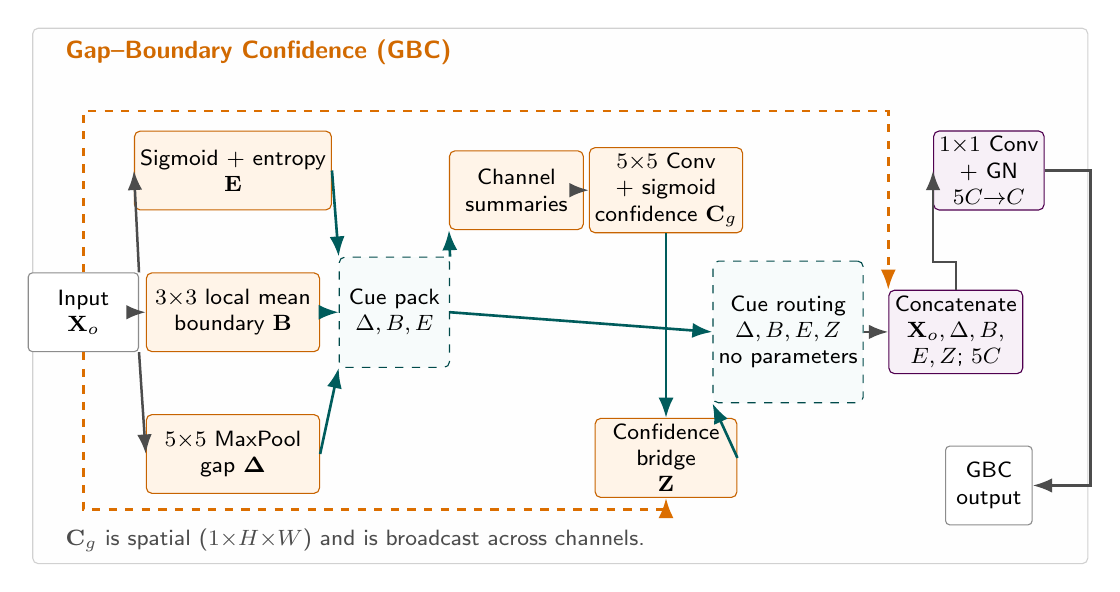
\begin{tikzpicture}[
  x=1cm,
  y=1cm,
  font=\sffamily\footnotesize,
  >=Latex,
  flow/.style={->, line width=0.9pt, draw=black!70},
  cue/.style={->, line width=0.95pt, draw=teal!72!black},
  skip/.style={->, line width=0.95pt, dashed, draw=orange!86!black},
  panel/.style={draw=black!18, rounded corners=2pt, fill=black!0.5},
  io/.style={draw=black!45, fill=white, rounded corners=1.5pt,
    minimum width=14mm, minimum height=10mm, align=center, inner sep=2pt},
  op/.style={draw=orange!78!black, fill=orange!9, rounded corners=2pt,
    minimum height=10mm, align=center, inner sep=2pt},
  routing/.style={draw=teal!58!black, dashed, fill=teal!3, rounded corners=2pt,
    minimum width=16mm, minimum height=24mm, align=center, inner sep=2pt},
  fusion/.style={draw=violet!62!black, fill=violet!6, rounded corners=2pt,
    minimum height=10mm, align=center, inner sep=2pt},
  note/.style={font=\sffamily\footnotesize, text=black!70}
]

\node[panel, minimum width=134mm, minimum height=68mm, anchor=south west]
  at (0.05,0.05) {};
\node[font=\sffamily\small\bfseries, text=orange!82!black, anchor=west]
  at (0.35,6.55) {Gap--Boundary Confidence (GBC)};

\node[io] (x) at (0.70,3.25) {Input\\$\mathbf{X}_o$};
\node[op, minimum width=22mm] (entropy) at (2.60,5.05)
  {Sigmoid + entropy\\$\mathbf{E}$};
\node[op, minimum width=22mm] (boundary) at (2.60,3.25)
  {$3{\times}3$ local mean\\boundary $\mathbf{B}$};
\node[op, minimum width=22mm] (gap) at (2.60,1.45)
  {$5{\times}5$ MaxPool\\gap $\boldsymbol{\Delta}$};
\node[routing, minimum width=14mm, minimum height=14mm] (pack) at (4.65,3.25)
  {Cue pack\\$\Delta,B,E$};
\node[op, minimum width=17mm] (summary) at (6.20,4.80)
  {Channel\\summaries};
\node[op, minimum width=18mm] (confidence) at (8.10,4.80)
  {$5{\times}5$ Conv\\+ sigmoid\\confidence $\mathbf{C}_g$};
\node[op, minimum width=18mm] (bridge) at (8.10,1.40)
  {Confidence\\bridge\\$\mathbf{Z}$};
\node[routing, minimum width=14mm, minimum height=18mm] (bus) at (9.65,3.00)
  {Cue routing\\$\Delta,B,E,Z$\\no parameters};
\node[fusion, minimum width=17mm] (concat) at (11.78,3.00)
  {Concatenate\\$\mathbf{X}_o,\Delta,B,$\\$E,Z$; $5C$};
\node[fusion, minimum width=14mm] (fuse) at (12.20,5.05)
  {$1{\times}1$ Conv\\+ GN\\$5C{\to}C$};
\node[io, minimum width=11mm] (out) at (12.20,1.05)
  {GBC\\output};

\draw[flow] (x.north east) -- (entropy.west);
\draw[flow] (x.east) -- (boundary.west);
\draw[flow] (x.south east) -- (gap.west);
\draw[cue] (entropy.east) -- (pack.north west);
\draw[cue] (boundary.east) -- (pack.west);
\draw[cue] (gap.east) -- (pack.south west);
\draw[cue] (pack.north east) -- (summary.south west);
\draw[flow] (summary) -- (confidence);
\draw[cue] (confidence) -- (bridge);
\draw[cue] (pack.east) -- (bus.west);
\draw[skip] (x.south) -- ++(0,-2.00) -| (bridge.south);
\draw[cue] (bridge.east) -- (bus.south west);
\draw[flow] (bus) -- (concat);
\draw[skip] (x.north) -- ++(0,2.05) -| (concat.north west);
\draw[flow] (concat.north) -- ++(0,0.35) -| (fuse.west);
\draw[flow] (fuse.east) -- ++(0.58,0) |- (out.east);

\node[note, anchor=west] at (0.35,0.35)
  {$\mathbf{C}_g$ is spatial ($1{\times}H{\times}W$) and is broadcast across channels.};

\end{tikzpicture}
\endgroup

\caption{Implementation-level GBC data flow. Gap, boundary, and entropy cues produce the spatial confidence map and bridge feature. The dashed cue-routing box is non-parametric and makes explicit the tensors collected by the final $5C$-channel fusion; the orange paths carry unchanged features.}
\label{fig:gbc_detail}
\end{figure}

\subsection{Training Objective}

The proposed model uses exactly the same loss as its controlled baseline. For a predicted crack probability $\hat{\mathbf{Y}}$ and binary label $\mathbf{Y}$, the objective is
\begin{equation}
\mathcal{L}=0.87\mathcal{L}_{\mathrm{BCE}}+0.13\mathcal{L}_{\mathrm{Dice}}.
\label{eq:loss}
\end{equation}
No auxiliary edge, topology, or module-specific loss is introduced. Therefore, the measured difference isolates the architectural refinement under a shared optimization objective.

\section{Experimental Setup}
\label{sec:experimental_setup}

\subsection{Datasets}

We evaluate on three public crack-segmentation benchmarks available in the project: CrackMap, DeepCrack, and CamCrack789~\cite{zou2019deepcrack,zhu2024lightweight,zhao2026mixercseg}. We use the fixed project splits without resampling. The available DeepCrack release contains 527 valid image--mask pairs; Table~\ref{tab:datasets} reports the exact paired files used rather than a nominal count from another release. Images and masks are resized to $512\times512$ with cubic interpolation, after which masks are binarized at 127. No random crop, flip, color, or geometric augmentation is applied by the dataset loader. CrackMap is used for paired multi-seed evaluation and full factorial ablation; DeepCrack and CamCrack789 provide single-seed transfer checks under the same training and evaluation implementation.

\begin{table}[H]
\centering
\caption{Dataset partitions used in the reported experiments.}
\label{tab:datasets}
\begin{tabular}{lrrrr}
\toprule
Dataset & Train & Validation & Test & Total \\
\midrule
CrackMap & 84 & 12 & 24 & 120 \\
DeepCrack & 368 & 53 & 106 & 527 \\
CamCrack789 & 553 & 79 & 157 & 789 \\
\bottomrule
\end{tabular}
\end{table}

\subsection{Implementation Details}

Both the baseline and proposed model are trained for 50 epochs with batch size 1. AdamW is used with an initial learning rate of $5\times10^{-4}$, weight decay 0.01, a PolyLR scheduler, and minimum learning rate $10^{-6}$. The loss weights are fixed to 0.87 for BCE and 0.13 for Dice, and all three datasets use 180 direction bins in DEGConv. No data split, preprocessing path, decoder setting, loss term, or optimization parameter is changed between the two models.

We report four paired CrackMap seeds: 42, 3407, 2026, and 1234. Pairing means that the baseline and proposed model use the same seed and training configuration. For every trajectory, all 50 checkpoints are evaluated on the validation split at threshold 0.5. The checkpoint with the highest validation mIoU is selected, with F1 and then the earlier epoch used as tie breakers. The test split is evaluated once after this selection. DeepCrack and CamCrack789 use seed 42 and the same validation-only rule. Training and profiling use NVIDIA GeForce RTX 3090 GPUs. Complexity is measured at input size $1\times3\times512\times512$ after 20 warm-up iterations and over 100 timed forward passes.

\subsection{Evaluation Metrics}

Predictions are saved as sigmoid probability maps and re-evaluated by one offline script. At the fixed threshold $t=0.5$, global confusion counts are used to compute precision, recall, F1, crack IoU, background IoU, and their mean:
\begin{align}
\mathrm{F1} &= \frac{2PR}{P+R}, \\
\mathrm{mIoU} &= \frac{1}{2}\left(
\frac{TP}{TP+FP+FN}+\frac{TN}{TN+FP+FN}\right).
\end{align}
ODS-F1 is the best dataset-level F1 obtained by sweeping thresholds from 0.00 to 0.99 in steps of 0.01. OIS-F1 selects the best threshold independently for each image and averages the resulting F1 scores. Mean and sample standard deviation are reported over seeds. For paired differences, we additionally report a two-sided $t$ interval with three degrees of freedom. Because only four seeds are available, these intervals are descriptive evidence of stability rather than a substitute for cross-dataset validation.

\section{Results and Discussion}
\label{sec:results}

\subsection{Paired Multi-Seed Results on CrackMap}

Table~\ref{tab:seed_results} lists every paired run after validation-only checkpoint selection. The proposed model improves fixed-threshold mIoU, fixed-threshold F1, ODS-F1, and OIS-F1 for all four seeds. The mIoU gain ranges from 0.0015 to 0.0520. The relatively large seed-to-seed variation, especially for the baseline, motivates reporting every paired result rather than only the strongest run.

% Source: work_dirs/20260919_085924_paper_v7_val_reselect_drop4_gpu12/reselected.metrics.tsv
\begin{table}[H]
\centering
\caption{Per-seed CrackMap results under the shared evaluation protocol.}
\label{tab:seed_results}
\resizebox{\textwidth}{!}{%
\begin{tabular}{rllcccc}
\toprule
Seed & Model & Mode & mIoU@0.5 & F1@0.5 & ODS-F1 & OIS-F1 \\
\midrule
42 & Baseline & -- & 0.7870 & 0.7447 & 0.7528 & 0.7501 \\
42 & Proposed & \method & \textbf{0.7993} & \textbf{0.7623} & \textbf{0.7881} & \textbf{0.7999} \\
\midrule
3407 & Baseline & -- & 0.7576 & 0.6978 & 0.6988 & 0.7234 \\
3407 & Proposed & \method & \textbf{0.8095} & \textbf{0.7766} & \textbf{0.7836} & \textbf{0.7860} \\
\midrule
2026 & Baseline & -- & 0.7994 & 0.7625 & 0.7685 & 0.7655 \\
2026 & Proposed & \method & \textbf{0.8217} & \textbf{0.7935} & \textbf{0.8034} & \textbf{0.8116} \\
\midrule
1234 & Baseline & -- & 0.8052 & 0.7702 & 0.7735 & 0.7790 \\
1234 & Proposed & \method & \textbf{0.8067} & \textbf{0.7727} & \textbf{0.7878} & \textbf{0.7974} \\
\bottomrule
\end{tabular}}
\end{table}

The aggregate comparison is shown in Table~\ref{tab:summary_results}. Mean mIoU increases by 0.0220, F1 by 0.0325, ODS-F1 by 0.0423, and OIS-F1 by 0.0442. The proposed model has a smaller across-seed standard deviation for every metric. Fixed-threshold precision rises from $0.6580\pm0.0313$ to $0.6895\pm0.0238$, and recall rises from $0.8576\pm0.0600$ to $0.8887\pm0.0070$. With only four pairs, the descriptive 95\% intervals for mIoU, F1, and ODS cross zero; only the OIS interval excludes zero. We therefore interpret the four positive paired outcomes as stability evidence, not as a claim of statistical significance.

% Source: work_dirs/20260919_085924_paper_v7_val_reselect_drop4_gpu12/crackmap_4seed.tsv
\begin{table}[H]
\centering
\caption{Four-seed CrackMap summary. Baseline and proposed values are mean$\pm$std; the interval is computed from paired seed differences.}
\label{tab:summary_results}
\resizebox{\textwidth}{!}{%
\begin{tabular}{lcccc}
\toprule
Metric & Baseline & Proposed & Mean gain & 95\% paired interval \\
\midrule
mIoU@0.5 & $0.7873\pm0.0212$ & $\mathbf{0.8093\pm0.0093}$ & $+0.0220$ & $[-0.0125,\,0.0565]$ \\
F1@0.5 & $0.7438\pm0.0325$ & $\mathbf{0.7763\pm0.0130}$ & $+0.0325$ & $[-0.0200,\,0.0850]$ \\
ODS-F1 & $0.7484\pm0.0342$ & $\mathbf{0.7907\pm0.0087}$ & $+0.0423$ & $[-0.0054,\,0.0900]$ \\
OIS-F1 & $0.7545\pm0.0238$ & $\mathbf{0.7987\pm0.0105}$ & $+0.0442$ & $[0.0146,\,0.0738]$ \\
\bottomrule
\end{tabular}}
\end{table}

The larger ODS/OIS gains indicate that the representation improves separability across thresholds in addition to the fixed 0.5 operating point. The lower standard deviations suggest reduced seed sensitivity, although the small number of seeds prevents a strong inferential claim.

\subsection{Context against Published CrackMap Results}

Table~\ref{tab:published_context} provides context from the original MixerCSeg comparison table. The external rows are published values and are not re-evaluated by our validation-selection and offline-metric pipeline; consequently, they are not a strict controlled ranking. In particular, the validation-selected proposed mIoU is not higher than every published number. The primary controlled comparison remains the paired baseline in Tables~\ref{tab:seed_results} and~\ref{tab:summary_results}.

\begin{table}[H]
\centering
\caption{CrackMap context. Published external values use their reported protocols; the proposed row is the four-seed mean from this project.}
\label{tab:published_context}
\begin{tabular}{lcccc}
\toprule
Method & mIoU & ODS & OIS & F1 \\
\midrule
SCSegamba~\cite{liu2025scsegamba} & 0.8094 & 0.7741 & 0.7766 & 0.7678 \\
MixerCSeg~\cite{zhao2026mixercseg} & 0.8123 & 0.7781 & 0.7806 & 0.7817 \\
Proposed \method & 0.8093 & 0.7907 & 0.7987 & 0.7763 \\
\bottomrule
\end{tabular}
\end{table}

\subsection{Cross-Dataset Validation}

Table~\ref{tab:cross_dataset} reports controlled seed-42 transfer results on DeepCrack and CamCrack789. Both methods use the same split, optimization settings, validation-only checkpoint rule, and offline metric implementation within each dataset. The proposed model improves all four metrics on CamCrack789. On DeepCrack, mIoU and F1 are lower by 0.0024 and 0.0027, respectively, and ODS/OIS are also slightly lower. The evidence therefore supports dataset-dependent transfer rather than universal improvement.

\begin{table}[H]
\centering
\caption{Controlled cross-dataset evaluation. CrackMap values are four-seed means; DeepCrack and CamCrack789 use seed 42. Bold marks the better controlled result within each dataset.}
\label{tab:cross_dataset}
\resizebox{\textwidth}{!}{%
\begin{tabular}{llcccc}
\toprule
Dataset & Model & mIoU & F1 & ODS-F1 & OIS-F1 \\
\midrule
CrackMap & Baseline & 0.7873 & 0.7438 & 0.7484 & 0.7545 \\
CrackMap & Proposed & \textbf{0.8093} & \textbf{0.7763} & \textbf{0.7907} & \textbf{0.7987} \\
\midrule
DeepCrack & Baseline & \textbf{0.9136} & \textbf{0.9097} & \textbf{0.9098} & \textbf{0.9110} \\
DeepCrack & Proposed & 0.9112 & 0.9070 & 0.9088 & 0.9080 \\
\midrule
CamCrack789 & Baseline & 0.8477 & 0.8278 & 0.8292 & 0.8354 \\
CamCrack789 & Proposed & \textbf{0.8570} & \textbf{0.8397} & \textbf{0.8397} & \textbf{0.8471} \\
\bottomrule
\end{tabular}}
\end{table}

\section{Ablation Study}
\label{sec:ablation}

The three modules form a full $2^3$ factorial design. An identity control retains the shared TripleStack wrapper and final residual gate while disabling MSA, OCV, and GBC. This control separates the wrapper from the three geometry components. The original MixerCSeg baseline is reported as an additional row without the wrapper. All configurations in Table~\ref{tab:ablation} were trained for 50 epochs with seed 42. Each checkpoint was selected on the 12-image validation split, after which the selected checkpoint was evaluated once on the same 24-image CrackMap test split. This controlled rerun is separate from the four-seed experiment, so its values are used only for within-table comparisons.

% Source: work_dirs/20260919_173408_v3_factorial_reselect9_gpu012/ablation.tsv
\begin{table}[H]
\centering
\caption{Complete seed-42 MSA/OCV/GBC component ablation on CrackMap. Best values are shown in bold.}
\label{tab:ablation}
\resizebox{\textwidth}{!}{%
\begin{tabular}{lcccccccc}
\toprule
Configuration & Wrapper & MSA & OCV & GBC & mIoU & F1 & ODS-F1 & OIS-F1 \\
\midrule
Original baseline & -- & -- & -- & -- & 0.7869 & 0.7443 & 0.7523 & 0.7497 \\
Identity control & \checkmark & -- & -- & -- & 0.7590 & 0.7035 & 0.7141 & 0.7096 \\
MSA only & \checkmark & \checkmark & -- & -- & 0.7959 & 0.7574 & 0.7641 & 0.7638 \\
OCV only & \checkmark & -- & \checkmark & -- & 0.8082 & 0.7748 & 0.7849 & 0.7956 \\
GBC only & \checkmark & -- & -- & \checkmark & 0.4849 & 0.0000 & 0.0586 & 0.0585 \\
MSA + OCV & \checkmark & \checkmark & \checkmark & -- & 0.7299 & 0.6572 & 0.6979 & 0.6966 \\
MSA + GBC & \checkmark & \checkmark & -- & \checkmark & 0.8125 & 0.7808 & 0.7820 & 0.7817 \\
OCV + GBC & \checkmark & -- & \checkmark & \checkmark & \textbf{0.8128} & \textbf{0.7810} & 0.7893 & 0.7974 \\
Full model & \checkmark & \checkmark & \checkmark & \checkmark & 0.8033 & 0.7681 & \textbf{0.7909} & \textbf{0.8007} \\
\bottomrule
\end{tabular}}
\end{table}

The identity wrapper is 2.79 mIoU points below the original baseline, so the gain cannot be attributed to the wrapper. MSA alone improves on the original baseline by 0.90 mIoU points and 1.30 F1 points, while OCV alone gives the clearest isolated gain of 2.13 and 3.04 points. GBC alone collapses to an all-background prediction at threshold 0.5, with validation selection retaining epoch 0. This negative result is kept because it shows that GBC is not a stable stand-alone feature extractor.

The pairwise results clarify the conditional role of GBC. Coupling it with MSA reaches 0.8125 mIoU, while OCV--GBC gives the highest fixed-threshold mIoU and F1 at 0.8128 and 0.7810. The complete chain improves over the original baseline by 1.65 mIoU points and 2.38 F1 points and gives the highest ODS/OIS at 0.7909/0.8007. Relative to OCV--GBC, adding MSA lowers fixed-threshold mIoU/F1 by 0.0094/0.0129 but raises ODS/OIS by 0.0016/0.0033. Thus, the full chain is not the fixed-threshold winner; its advantage is better threshold-swept separability. The poor validation-selected MSA--OCV result and the GBC-only collapse further show that these single-seed combinations are strongly coupled and should not be presented as independently additive effects.

\section{Complexity Analysis}
\label{sec:complexity}

Table~\ref{tab:complexity} reports measured complexity. The full method adds 0.517M parameters and 0.408 GFLOPs, corresponding to increases of 20.3\% and 20.5\%, respectively. Actual latency rises from 169.563 to 177.051 ms per image (4.4\%), and peak allocated GPU memory rises by approximately 1.0\%. This gap between theoretical operation count and measured latency occurs because most added operations are depthwise convolution, fixed channel-wise filtering, pooling, and pointwise fusion.

% Source: logs/20260806_220017_CrackMap_triple_stack_v4_search12_validate8_gpu0.profile.log
\begin{table}[H]
\centering
\caption{Complexity at $512\times512$ input resolution and batch size 1.}
\label{tab:complexity}
\resizebox{\textwidth}{!}{%
\begin{tabular}{lrrrrrr}
\toprule
Model & Params (M) & FLOPs (G) & Size (MB) & FPS & Latency (ms) & GPU memory (MB) \\
\midrule
Baseline & 2.542 & 1.989 & 9.715 & 5.898 & 169.563 & 195.798 \\
Proposed \method & 3.059 & 2.397 & 11.686 & 5.648 & 177.051 & 197.820 \\
\midrule
Relative change & +20.3\% & +20.5\% & +20.3\% & $-4.2\%$ & +4.4\% & +1.0\% \\
\bottomrule
\end{tabular}}
\end{table}

The overhead is larger than that of the original lightweight DEGConv alone, so the method should not be described as cost-free. The measured CrackMap and CamCrack789 gains support this trade-off, but the slight DeepCrack regression shows that the additional capacity does not guarantee transfer to every crack domain.

\section{Qualitative Analysis}
\label{sec:qualitative}

Figures~\ref{fig:qualitative_predictions} and~\ref{fig:qualitative_errors} compare the validation-selected seed-42 baseline and full \method{} checkpoints at the same fixed threshold of 0.5 used for the reported fixed-threshold metrics. To avoid selecting examples according to which model looked better, the four cases were chosen deterministically from ground-truth morphology alone. The rules select a sparse mask, a fragmented mask, a mask with high boundary complexity, and a relatively dense mask. Within each image, a fixed-size zoom region maximizes ground-truth crack pixels; ties are resolved by proximity to the ground-truth centroid. Predictions do not participate in either selection step. Image identifiers, crop coordinates, rule values, file paths, and SHA-256 hashes are recorded in the accompanying manifest. The examples expose mixed behavior rather than only favorable cases: the proposed model preserves more weak elongated pixels in several regions, but residual false positives and missed fine branches remain visible.

% Generated by tools/make_paper_qualitative_v2.py.
% Manifest: figures/qualitative_selection_v2.tsv
\begin{figure}[H]
\centering
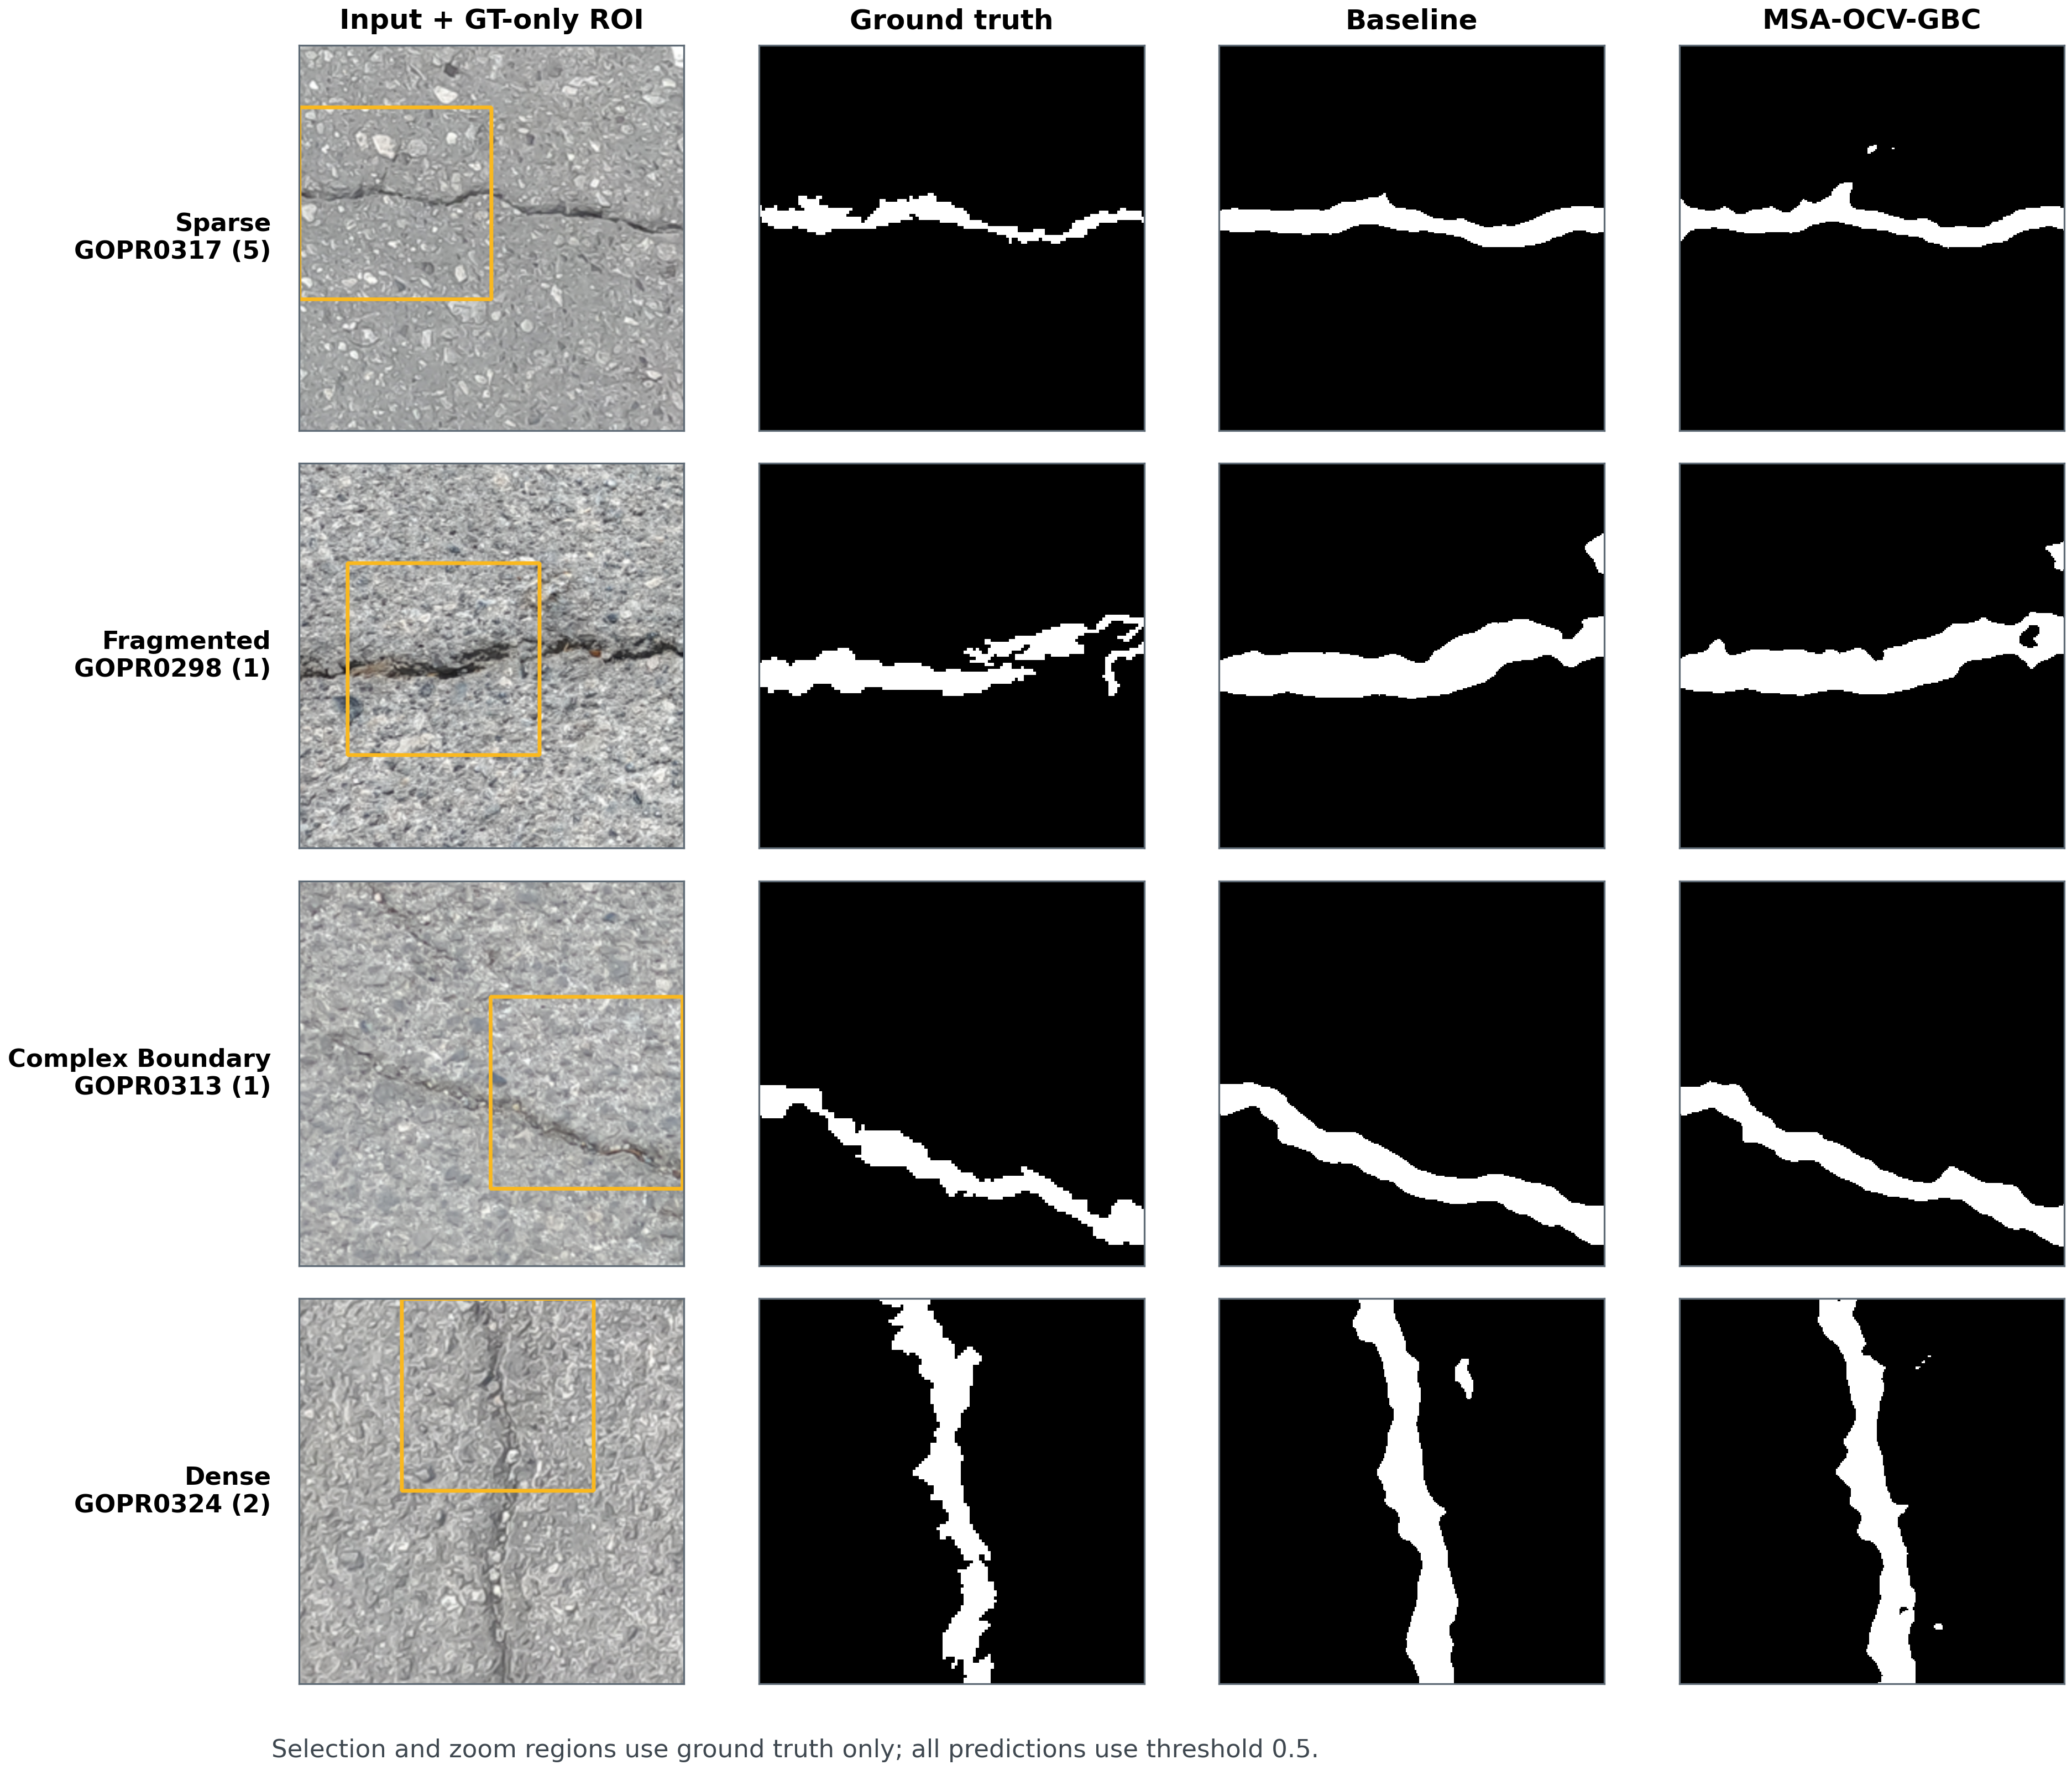
\includegraphics[width=\textwidth]{figures/qualitative_predictions_v2.png}
\caption{Controlled prediction comparison on CrackMap. The first column shows the full image and its ground-truth-defined zoom box; the remaining columns enlarge that same region. Rows represent sparse, fragmented, complex-boundary, and dense masks. Both models use threshold 0.5.}
\label{fig:qualitative_predictions}
\end{figure}

\begin{figure}[H]
\centering
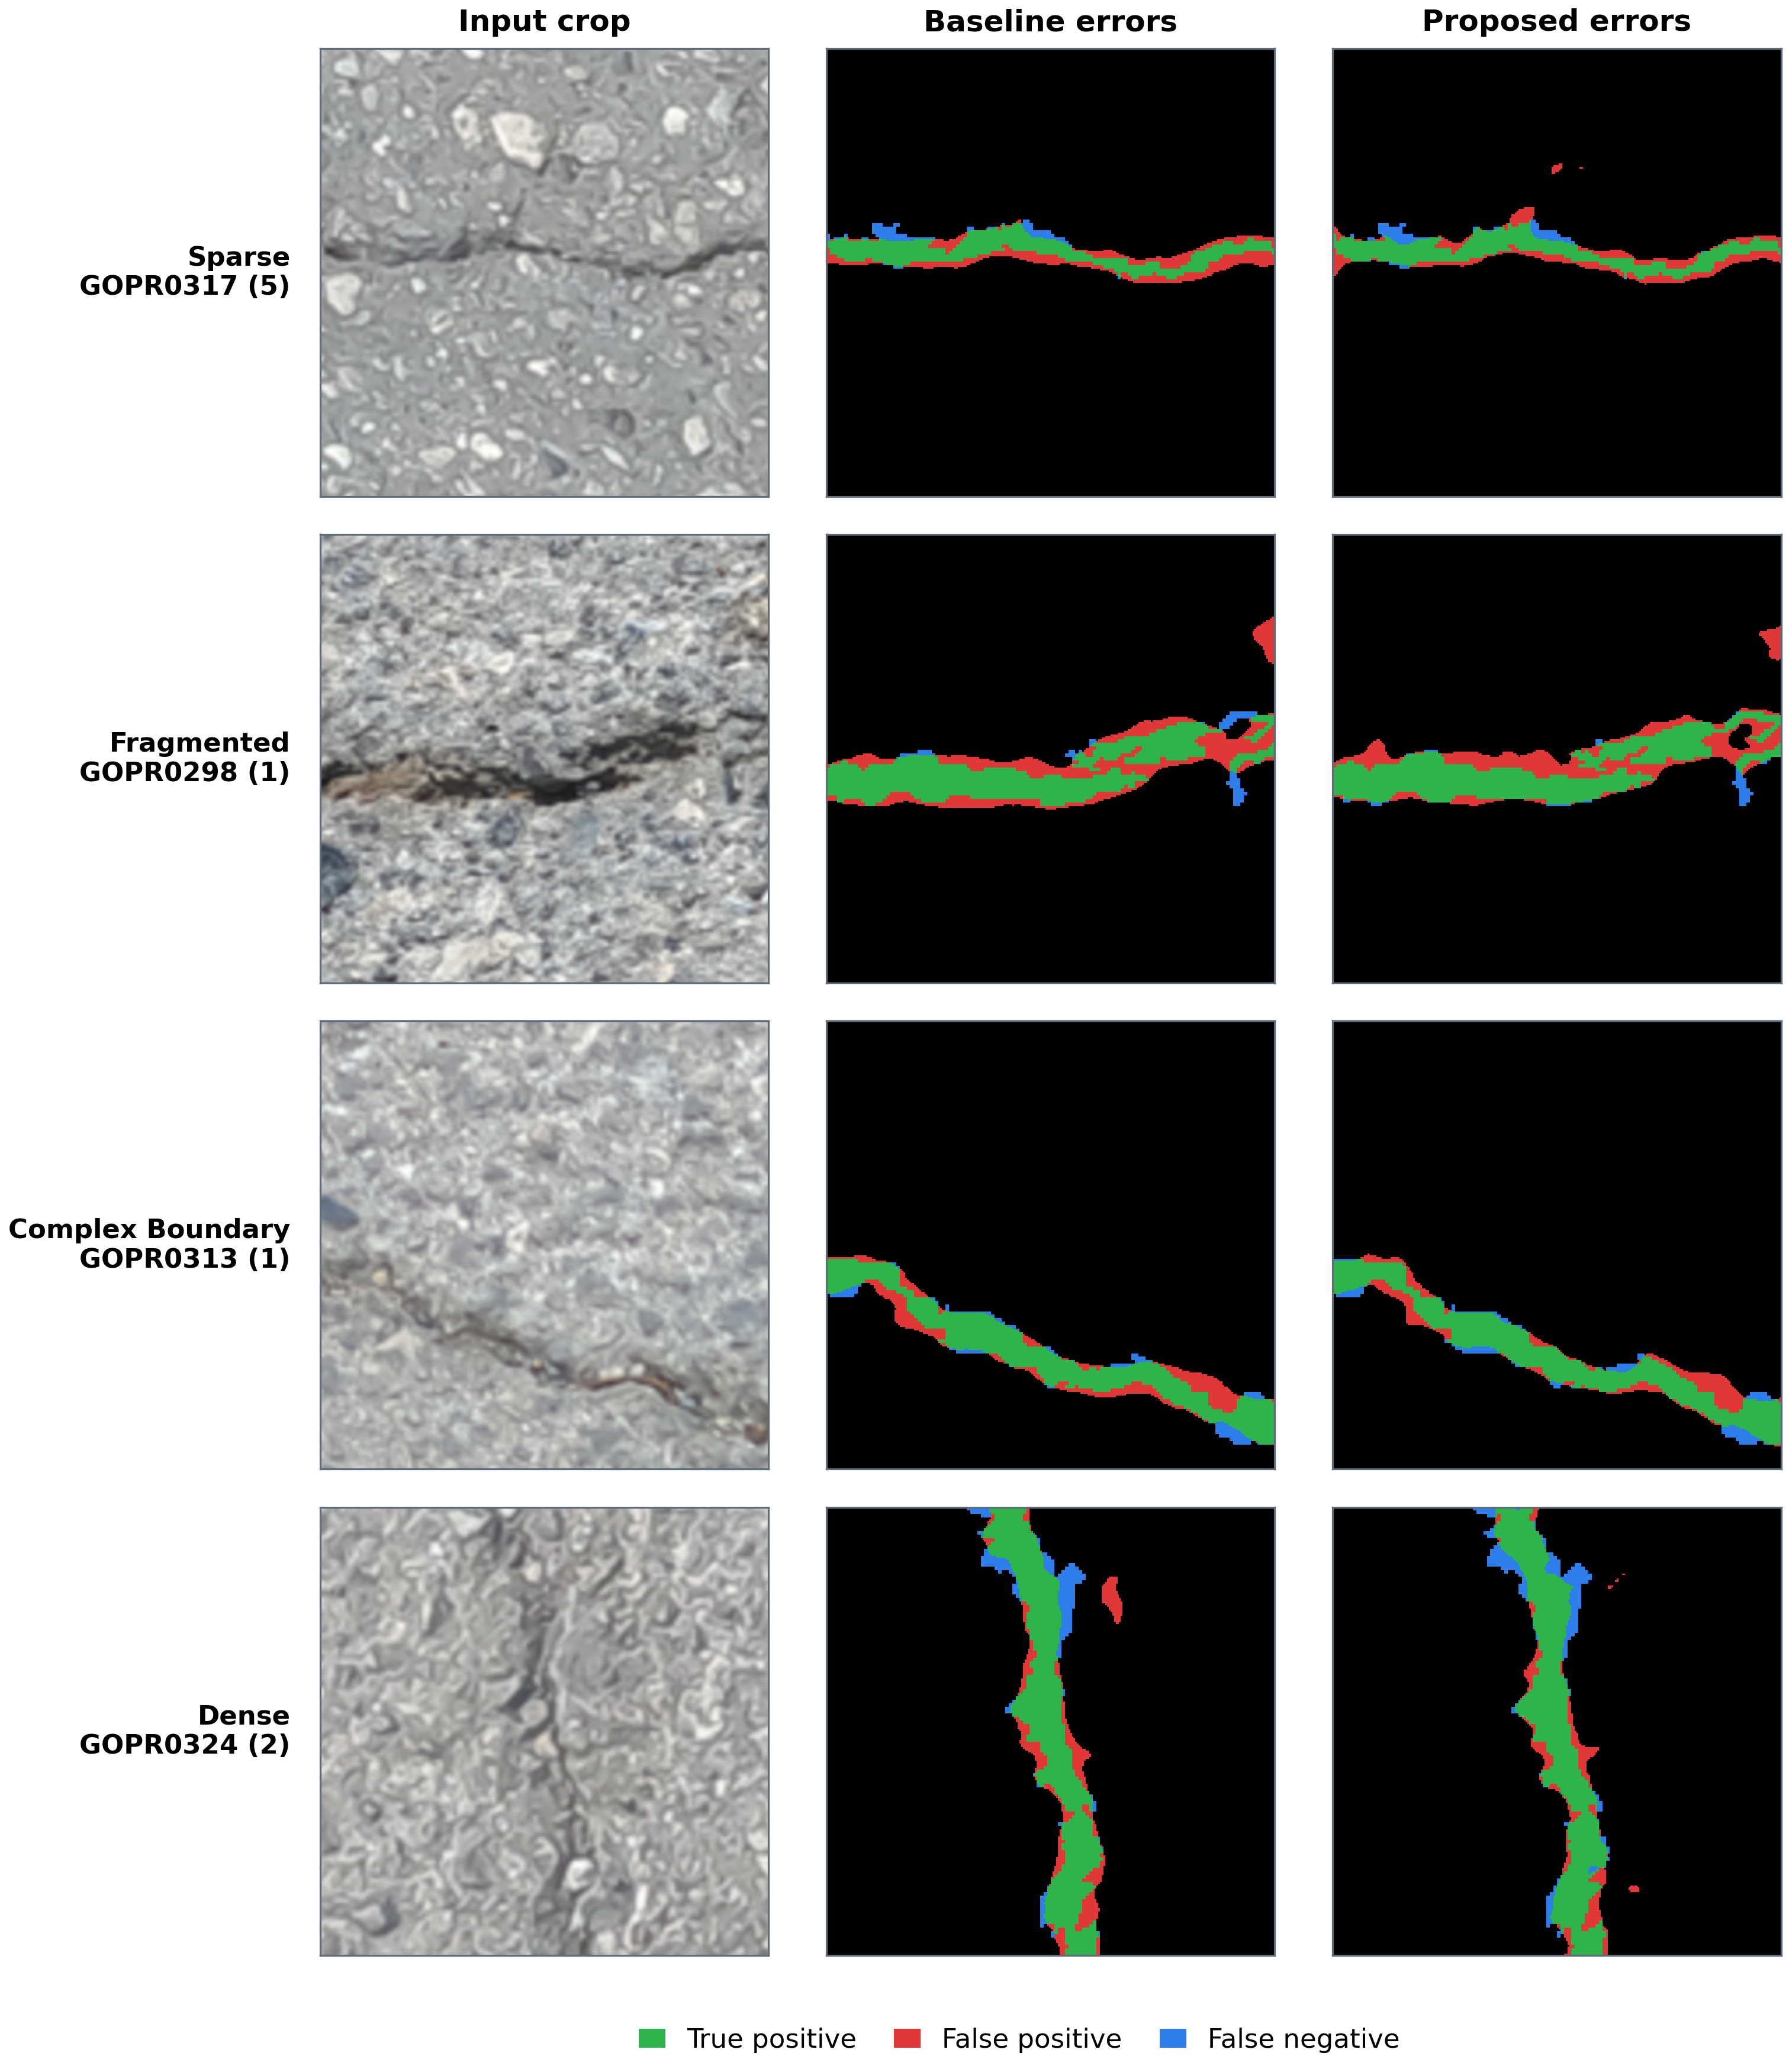
\includegraphics[width=\textwidth]{figures/qualitative_errors_v2.png}
\caption{Enlarged error maps for the same samples and ground-truth-defined regions as Fig.~\ref{fig:qualitative_predictions}. Green denotes true positives, red false positives, and blue false negatives. The comparison retains both favorable and unfavorable outcomes.}
\label{fig:qualitative_errors}
\end{figure}

\section{Limitations}

The current evidence has five limitations. First, the multi-seed evaluation covers only CrackMap; DeepCrack and CamCrack789 each use one seed. The proposed model improves CamCrack789 but is slightly below the baseline on DeepCrack, so broad cross-domain superiority is not established. Crack500 was not evaluated under the final protocol. Second, the factorial ablation uses one seed. Its differences are useful for diagnosing component interactions but should not be interpreted as stable or statistically significant effects. In particular, OCV--GBC is better than the complete chain at the fixed threshold, GBC collapses in isolation, and MSA--OCV also underperforms the baseline. These outcomes do not support a claim that every component contributes independently. Third, the architecture emerged from extensive exploratory searches in which test-set metrics were repeatedly inspected. Validation-only checkpoint reselection removes test-based epoch selection from the reported runs, but it cannot retrospectively remove architecture-selection bias. Independent replication on unseen data is therefore needed. Fourth, the four paired seeds provide descriptive uncertainty only; the sample is too small for strong inferential claims. Finally, parameters and FLOPs rise by approximately 20\%, although measured latency and memory grow more slowly. OCV's fixed derivative kernels may not represent every texture-dependent orientation pattern, and GBC entropy is an intermediate ambiguity cue rather than calibrated predictive uncertainty.

\section{Conclusion}

This paper presents a geometry-aware extension of MixerCSeg organized around scale conditioning, orientation--curvature voting, and confidence-guided gap refinement. MSA combines multi-scale axial depthwise filters with global row and column context before DEGConv. OCV integrates Sobel magnitude, Hessian-derived ridge and curvature responses, and learnable directional filtering after DEGConv. GBC uses local gap, boundary, and entropy cues to control feature bridging. Gated residual integration coordinates the three stages without modifying the decoder or training objective. Under validation-only checkpoint selection, four paired CrackMap seeds improve mean mIoU, F1, ODS-F1, and OIS-F1 by 2.20, 3.25, 4.23, and 4.42 percentage points, respectively, with a 4.4\% measured latency increase. The single-seed factorial experiment identifies OCV--GBC as the best fixed-threshold configuration and the full chain as the best threshold-swept configuration, demonstrating meaningful but non-additive component interactions. Single-seed transfer is positive on CamCrack789 and slightly negative on DeepCrack. The results therefore support \method{} as a promising CrackMap-focused refinement, while the limited seed count, mixed transfer, and prior architecture-search exposure require conservative generalization claims.

\section*{Declaration of Competing Interest}

The authors declare that they have no known competing financial interests or personal relationships that could have appeared to influence the work reported in this paper.

\section*{Data and Code Availability}

The datasets are publicly available from their cited sources. The exact source code, configurations, checkpoint-selection records, probability-map manifests, and metric summaries used for this manuscript are preserved in the project repository. They can be provided to editors and reviewers during evaluation, subject to the datasets' redistribution terms. A permanent public repository URL will be added before publication when anonymity restrictions are lifted.

\begin{thebibliography}{00}

\bibitem{long2015fcn}
J. Long, E. Shelhamer, T. Darrell,
Fully convolutional networks for semantic segmentation,
in: Proceedings of the IEEE Conference on Computer Vision and Pattern Recognition, 2015, pp. 3431--3440.

\bibitem{ronneberger2015unet}
O. Ronneberger, P. Fischer, T. Brox,
U-Net: Convolutional networks for biomedical image segmentation,
in: Medical Image Computing and Computer-Assisted Intervention, 2015, pp. 234--241.

\bibitem{shi2016crackforest}
Y. Shi, L. Cui, Z. Qi, F. Meng, Z. Chen,
Automatic road crack detection using random structured forests,
IEEE Transactions on Intelligent Transportation Systems 17 (12) (2016) 3434--3445.

\bibitem{zou2019deepcrack}
Q. Zou, Z. Zhang, Q. Li, X. Qi, Q. Wang, S. Wang,
DeepCrack: Learning hierarchical convolutional features for crack detection,
IEEE Transactions on Image Processing 28 (3) (2019) 1498--1512.

\bibitem{guo2021barnet}
J.-M. Guo, H. Markoni, J.-D. Lee,
BARNet: Boundary aware refinement network for crack detection,
IEEE Transactions on Intelligent Transportation Systems 23 (7) (2022) 7343--7358.

\bibitem{xiang2023dtrcnet}
C. Xiang, J. Guo, R. Cao, L. Deng,
A crack-segmentation algorithm fusing transformers and convolutional neural networks for complex detection scenarios,
Automation in Construction 152 (2023) 104894.

\bibitem{gu2024mamba}
A. Gu, T. Dao,
Mamba: Linear-time sequence modeling with selective state spaces,
in: First Conference on Language Modeling, 2024.

\bibitem{liu2024vmamba}
Y. Liu, Y. Tian, Y. Zhao, H. Yu, L. Xie, Y. Wang, Q. Ye, J. Jiao, Y. Liu,
VMamba: Visual state space model,
Advances in Neural Information Processing Systems 37 (2024) 103031--103063.

\bibitem{he2024crackmamba}
Z. He, Y.-H. Wang,
Mamba meets crack segmentation,
arXiv preprint arXiv:2407.15714 (2024).

\bibitem{liu2025scsegamba}
H. Liu, C. Jia, F. Shi, X. Cheng, S. Chen,
SCSegamba: Lightweight structure-aware vision Mamba for crack segmentation in structures,
in: Proceedings of the IEEE/CVF Conference on Computer Vision and Pattern Recognition, 2025, pp. 29406--29416.

\bibitem{zhao2026mixercseg}
Z. Zhao, Z. Ding, P. Niu, W. Sun, F. Guo,
MixerCSeg: An efficient mixer architecture for crack segmentation via decoupled Mamba attention,
arXiv preprint arXiv:2603.01361 (2026).

\bibitem{hou2020strip}
Q. Hou, L. Zhang, M.-M. Cheng, J. Feng,
Strip pooling: Rethinking spatial pooling for scene parsing,
in: Proceedings of the IEEE/CVF Conference on Computer Vision and Pattern Recognition, 2020, pp. 4003--4012.

\bibitem{frangi1998vessel}
A. F. Frangi, W. J. Niessen, K. L. Vincken, M. A. Viergever,
Multiscale vessel enhancement filtering,
in: Medical Image Computing and Computer-Assisted Intervention, 1998, pp. 130--137.

\bibitem{yang2019crack500}
F. Yang, L. Zhang, S. Yu, D. Prokhorov, X. Mei, H. Ling,
Feature pyramid and hierarchical boosting network for pavement crack detection,
IEEE Transactions on Intelligent Transportation Systems 21 (4) (2020) 1525--1535.

\bibitem{zhu2024lightweight}
G. Zhu, J. Liu, Z. Fan, D. Yuan, P. Ma, M. Wang, W. Sheng, K. C. P. Wang,
A lightweight encoder--decoder network for automatic pavement crack detection,
Computer-Aided Civil and Infrastructure Engineering 39 (12) (2024) 1743--1765.

\end{thebibliography}

\end{document}
